\section{Oleaje}


Las olas marinas son consecuencia de la propagación del movimiento entre dos medios, el aire de la
atmósfera y el agua del mar. Los cambios de presión atmosférica provocan oscilaciones en la
superficie del líquido. A su vez, la acción del viento que roza la superficie da lugar a lo que se
conoce como ondas capilares, cuando su empuje es más leve, u ondas gravitatorias, cuando la
fricción sobre la lámina de agua es más intensa.

Podemos clasificar las olas en dos tipos:

\begin{enumerate}
\item \textbf{Olas de viento: }
Olas generadas por el viento. Generalmente, los vientos más fuertes provocan olas más altas. Entran en juego factores como la
velocidad e intensidad de la acción eólica, la cantidad de tiempo que el aire mantiene una dirección
estable, el área de la superficie del agua afectada y la profundidad. A medida que las olas se
acercan a la orilla, avanzan más despacio debido a que hay menos profundidad, mientras que la
cresta aumenta su altura. El proceso continúa hasta que la zona levantada se mueve más rápido
que la parte subacuática, punto en el que el movimiento se desestabiliza y la ola rompe.

 \item \textbf{Mar de fondo: } 
Mar de fondo es el movimiento de las olas (también llamado oleaje o
sistema de olas) que se propaga fuera de la zona donde se ha generado, pudiendo llegar a lugares
muy alejados. Por tanto este estado del mar no tiene relación con el viento presente, aunque su 
causa es el viento que se haya originado en otra área distinta. Las olas del mar de fondo se
caracterizan por su período regular y sus crestas suaves. La longitud de la onda es muy superior a su
altura, presentando crestas redondeadas que no rompen nunca en alta mar.

\end{enumerate}


El oleaje es otro de los factores a tener en cuenta cuando estamos en el mar. Necesitaremos también una forma de clasificar el estado de la mar en función de su oleaje, para ello utilizaremos la escala Douglas. \cite{DOUGLAS}


\begin{figure}[hb]
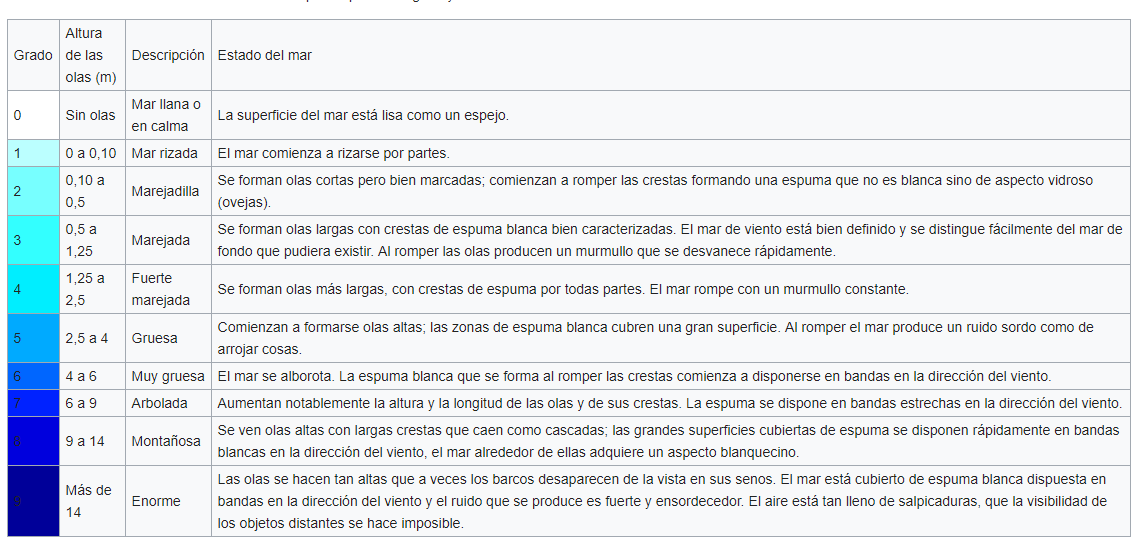
\includegraphics[scale=0.55]{escala_douglas.png} 
\floatfoot{Figura 2. Escala Douglas}
\end{figure}

A partir del grado 6 no es recomendable practicar deportes marinos como el windsurf, y aunque no vamos a tener en cuenta el oleaje para nuestra aplicación, si lo podemos incluir en el apartado de mejoras, añadiendo la suscripción de la aplicación a un servicio de alertas de mal tiempo, donde se verá reflejado el oleaje como uno de los indicadores para desaconsejar la práctica de deportes en el mar. 

